\newcommand{\dropperTagResultsAucTable}{
    \begin{table}[h!]
        \centering
        \begin{tabular}{|p{2,8cm}||P{2,2cm} P{2,2cm} P{2,2cm} P{2,2cm}|}
            \hline
            Dropper Tag & ALOHA\newline (M/B only) & ALOHA & Joint\newline Embedding & Proposed\newline Model \\
            \hline
            AUC-ROC & - & 0.972$\pm$0.001 & 0.973$\pm$0.001 & \textBF{0.976$\pm$0.001} \\
            \hline
        \end{tabular}
        \caption[Dropper Tag prediction task AUC-ROC results]{AUC-ROC (Area Under Curve) of the different models for the \textbf{Dropper Tag} prediction task. Results were aggregated over \textBF{3} training runs with different weight initializations and minibatch orderings. Best results are shown in \textbf{bold}.} \label{tab:dropperTag_auc}
    \end{table}
}

\newcommand{\dropperTagResultsAtFprTable}{
    \begin{center}
        \begin{longtable}[c]{|P{3,2cm}||P{1,8cm} P{1,8cm} P{1,8cm} P{1,8cm} P{1,8cm}|}
            \hline
            Dropper Tag & \multicolumn{5}{c|}{{FPR}} \\
            & $10^{-5}$ & $10^{-4}$ & $10^{-3}$ & $10^{-2}$ & $10^{-1}$ \\
            \hline
            \endfirsthead

            \caption*{\raggedright ...continued from previous page} \\
            \hline
            Dropper Tag & \multicolumn{5}{c|}{\textbf{FPR}} \\
            & $10^{-5}$ & $10^{-4}$ & $10^{-3}$ & $10^{-2}$ & $10^{-1}$ \\
            \hline
            \endhead

            \caption*{\raggedleft ...continued on next page} \\
            \endfoot

            \caption[Dropper Tag prediction task results]{Mean and standard deviation results (TPR, Accuracy, Recall, Precision and F1-Score) of the different models for the \textbf{Dropper Tag} prediction task at different \textbf{FPR}s (\textit{False Positive Rates}). Results were aggregated over \textBF{3} training runs with different weight initializations and minibatch orderings. Best results are shown in \textbf{bold}. Under \textbf{TPR} results are also presented the percentage reduction in mean detection error and in ROC curve standard deviation introduced by the \textit{Proposed Model} with respect to both \textit{ALOHA} model and \textit{Joint Embedding}.} \label{tab:dropperTag_results_at_fpr} \\
            \endlastfoot

            \multicolumn{6}{|c|}{\textbf{TPR}} \\
            \hline
            ALOHA (M/B only) & - & - & - & - & - \\
            ALOHA & 0.045$\pm$0.007 & 0.068$\pm$0.021 & 0.121$\pm$0.063 & 0.672$\pm$0.026 & 0.921$\pm$0.011 \\
            Joint Embedding & \textBF{0.118$\pm$0.078} & \textBF{0.159$\pm$0.132} & 0.179$\pm$0.131 & \textBF{0.730$\pm$0.011} & 0.910$\pm$0.015 \\
            Proposed Model & 0.042$\pm$0.020 & 0.128$\pm$0.051 & \textBF{0.206$\pm$0.076} & 0.724$\pm$0.016 & \textBF{0.933$\pm$0.015} \\
            \hline
            Error Reduction wrt\newline ALOHA (M/B only) & - & - & - & - & - \\
            Error Reduction wrt\newline ALOHA & -0.3\% & 6.4\% & 9.7\% & 15.9\% & 15.2\% \\
            Error Reduction wrt\newline Joint Embedding & -8.6\% & -3.7\% & 3.3\% & -2.2\% & 25.6\% \\
            \hline
            Std Reduction wrt\newline ALOHA (M/B only) & - & - & - & - & - \\
            Std Reduction wrt\newline ALOHA & -185.7\% & -142.9\% & -20.6\% & 38.5\% & -36.4\% \\
            Std Reduction wrt\newline Joint Embedding & 74.4\% & 61.4\% & 42.0\% & -45.5\% & 0.0\% \\
            \hline
            \multicolumn{6}{|c|}{\textbf{Accuracy}} \\
            \hline
            ALOHA (M/B only) & - & - & - & - & - \\
            ALOHA & 0.878$\pm$0.001 & 0.881$\pm$0.003 & 0.887$\pm$0.008 & 0.949$\pm$0.003 & 0.903$\pm$0.001 \\
            Joint Embedding & \textBF{0.887$\pm$0.010} & \textBF{0.893$\pm$0.017} & 0.894$\pm$0.017 & \textBF{0.957$\pm$0.001} & 0.901$\pm$0.002 \\
            Proposed Model & 0.878$\pm$0.003 & 0.889$\pm$0.007 & \textBF{0.898$\pm$0.010} & 0.956$\pm$0.002 & \textBF{0.904$\pm$0.002} \\
            \hline
            \multicolumn{6}{|c|}{\textbf{Recall}} \\
            \hline
            ALOHA (M/B only) & - & - & - & - & - \\
            ALOHA & 0.045$\pm$0.007 & 0.068$\pm$0.021 & 0.121$\pm$0.063 & 0.672$\pm$0.026 & 0.921$\pm$0.011 \\
            Joint Embedding & \textBF{0.118$\pm$0.078} & \textBF{0.159$\pm$0.132} & 0.179$\pm$0.131 & \textBF{0.730$\pm$0.011} & 0.910$\pm$0.015 \\
            Proposed Model & 0.042$\pm$0.020 & 0.128$\pm$0.051 & \textBF{0.206$\pm$0.076} & 0.724$\pm$0.016 & \textBF{0.933$\pm$0.015} \\
            \hline
            \multicolumn{6}{|c|}{\textbf{Precision}} \\
            \hline
            ALOHA (M/B only) & - & - & - & - & - \\
            ALOHA & \textBF{0.999$\pm$0.000} & 0.989$\pm$0.004 & 0.931$\pm$0.035 & 0.908$\pm$0.003 & 0.574$\pm$0.003 \\
            Joint Embedding & 0.999$\pm$0.001 & 0.992$\pm$0.005 & 0.944$\pm$0.029 & \textBF{0.914$\pm$0.001} & 0.571$\pm$0.004 \\
            Proposed Model & 0.998$\pm$0.001 & \textBF{0.994$\pm$0.002} & \textBF{0.963$\pm$0.015} & 0.914$\pm$0.002 & \textBF{0.577$\pm$0.004} \\
            \hline
            \multicolumn{6}{|c|}{\textbf{F1 Score}} \\
            \hline
            ALOHA (M/B only) & - & - & - & - & - \\
            ALOHA & 0.086$\pm$0.013 & 0.127$\pm$0.038 & 0.210$\pm$0.098 & 0.772$\pm$0.019 & 0.707$\pm$0.005 \\
            Joint Embedding & \textBF{0.203$\pm$0.121} & \textBF{0.253$\pm$0.186} & 0.282$\pm$0.177 & \textBF{0.812$\pm$0.007} & 0.702$\pm$0.007 \\
            Proposed Model & 0.080$\pm$0.036 & 0.222$\pm$0.079 & \textBF{0.332$\pm$0.106} & 0.808$\pm$0.011 & \textBF{0.713$\pm$0.007} \\
            \hline
        \end{longtable}
    \end{center}
}

\newcommand{\dropperTagResultsSummaryTable}{
    \begin{table}[h!]
        \centering
        \begin{tabular}{|P{3,2cm}||P{1,8cm} P{1,8cm} P{1,8cm} P{1,8cm} P{1,8cm}|}
            \hline
            \multicolumn{6}{|c|}{Dropper Tag (at FPR $=1\%$)} \\
            \hline
            Model & TPR & Accuracy & Precision & Recall & F1 score \\
            \hline
            ALOHA (M/B only) & - & - & - & - & - \\
            ALOHA & 0.672$\pm$0.026 & 0.949$\pm$0.003 & 0.908$\pm$0.003 & 0.672$\pm$0.026 & 0.772$\pm$0.019 \\
            Joint Embedding & \textBF{0.730$\pm$0.011} & \textBF{0.957$\pm$0.001} & \textBF{0.914$\pm$0.001} & \textBF{0.730$\pm$0.011} & \textBF{0.812$\pm$0.007} \\
            Proposed Model & 0.724$\pm$0.016 & 0.956$\pm$0.002 & 0.914$\pm$0.002 & 0.724$\pm$0.016 & 0.808$\pm$0.011 \\
            \hline
        \end{tabular}
        \caption[Summary of Dropper Tag prediction task results]{Summary of the mean and standard deviation results of the different models for the \textbf{Dropper Tag} prediction task at \textbf{FPR} $=1\%$. Results were aggregated over \textBF{3} training runs with different weight initializations and minibatch orderings. Best results are shown in \textbf{bold}.} \label{tab:dropperTag_result_summary}
    \end{table}
}

\newcommand{\dropperTagRocAlohaMB}{
    \begin{figure}[h!]
        \vspace*{-0.5cm}
        \centering
        \includegraphics[width=0.6\textwidth]{./results/dropper_tag_roc_alohaMB.png}
        \vspace*{-0.2cm}
        \caption[Dropper Tag prediction task ALOHA (M/B only) ROC curve]{ROC curve and AUC statistics of \textBF{ALOHA (M/B only)} model for the \textbf{Dropper Tag}. The line represents the \textit{mean} TPR at a given FPR, while the shaded region represents the \textit{standard deviation}. Statistics were computed over \textBF{3} training runs, each with random parameter initialization.}
        \label{fig:dropperTagRocAlohaMB}
    \end{figure}
}

\newcommand{\dropperTagRocAloha}{
    \begin{figure}[h!]
        \vspace*{-0.5cm}
        \centering
        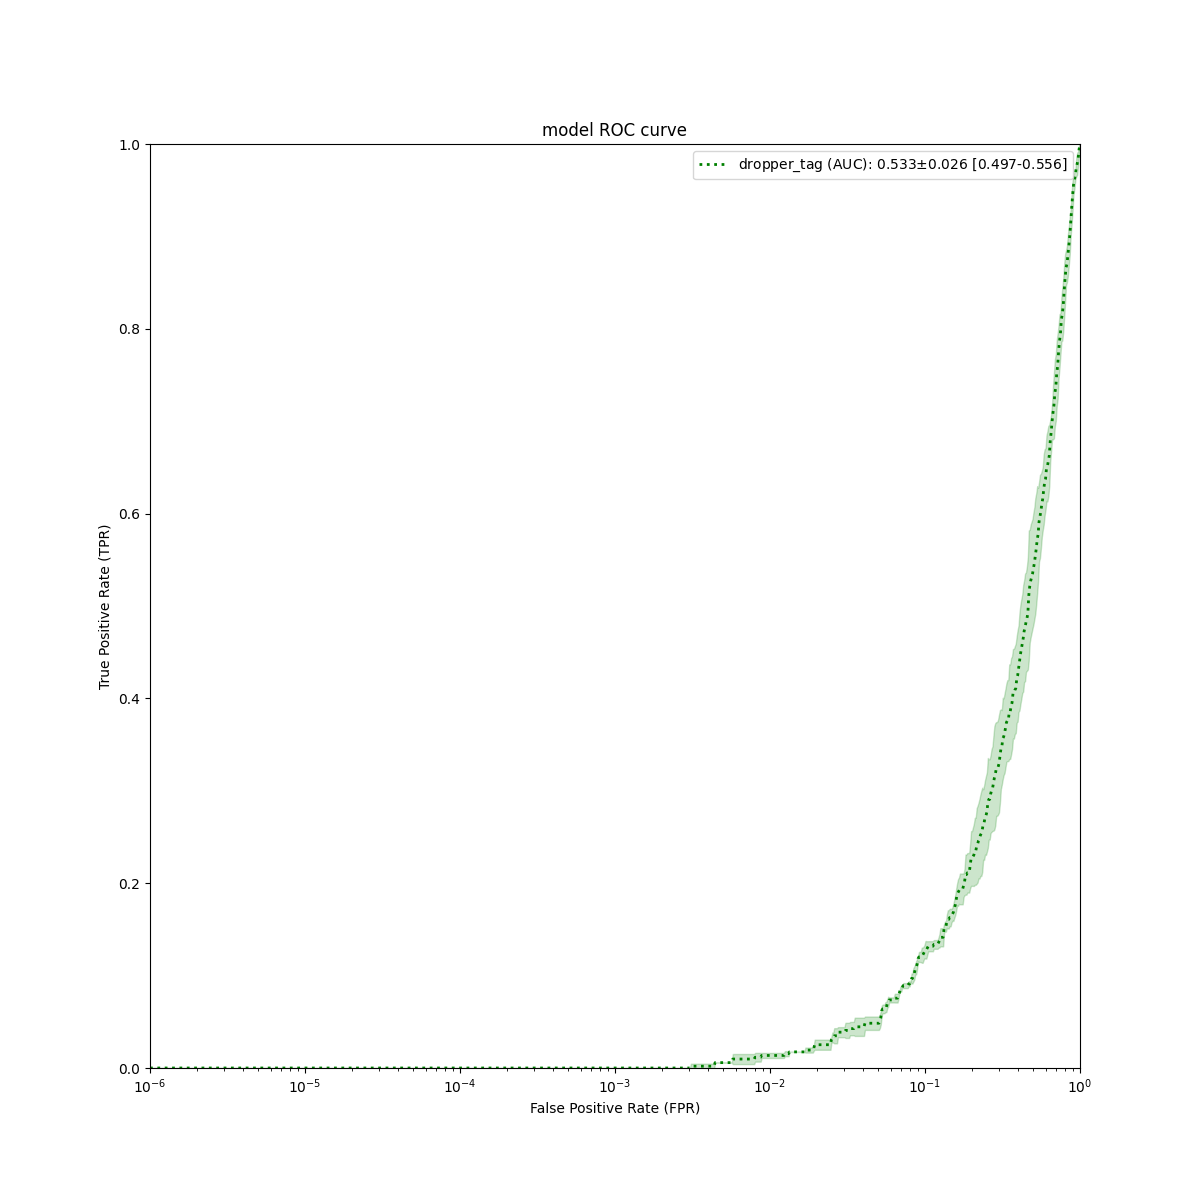
\includegraphics[width=0.6\textwidth]{./results/dropper_tag_roc_aloha.png}
        \vspace*{-0.2cm}
        \caption[Dropper Tag prediction task ALOHA ROC curve]{ROC curve and AUC statistics of \textBF{ALOHA} model for the \textbf{Dropper Tag}. The line represents the \textit{mean} TPR at a given FPR, while the shaded region represents the \textit{standard deviation}. Statistics were computed over \textBF{3} training runs, each with random parameter initialization.}
        \label{fig:dropperTagRocAloha}
    \end{figure}
}

\newcommand{\dropperTagRocJointEmbedding}{
    \begin{figure}[h!]
        \vspace*{-0.5cm}
        \centering
        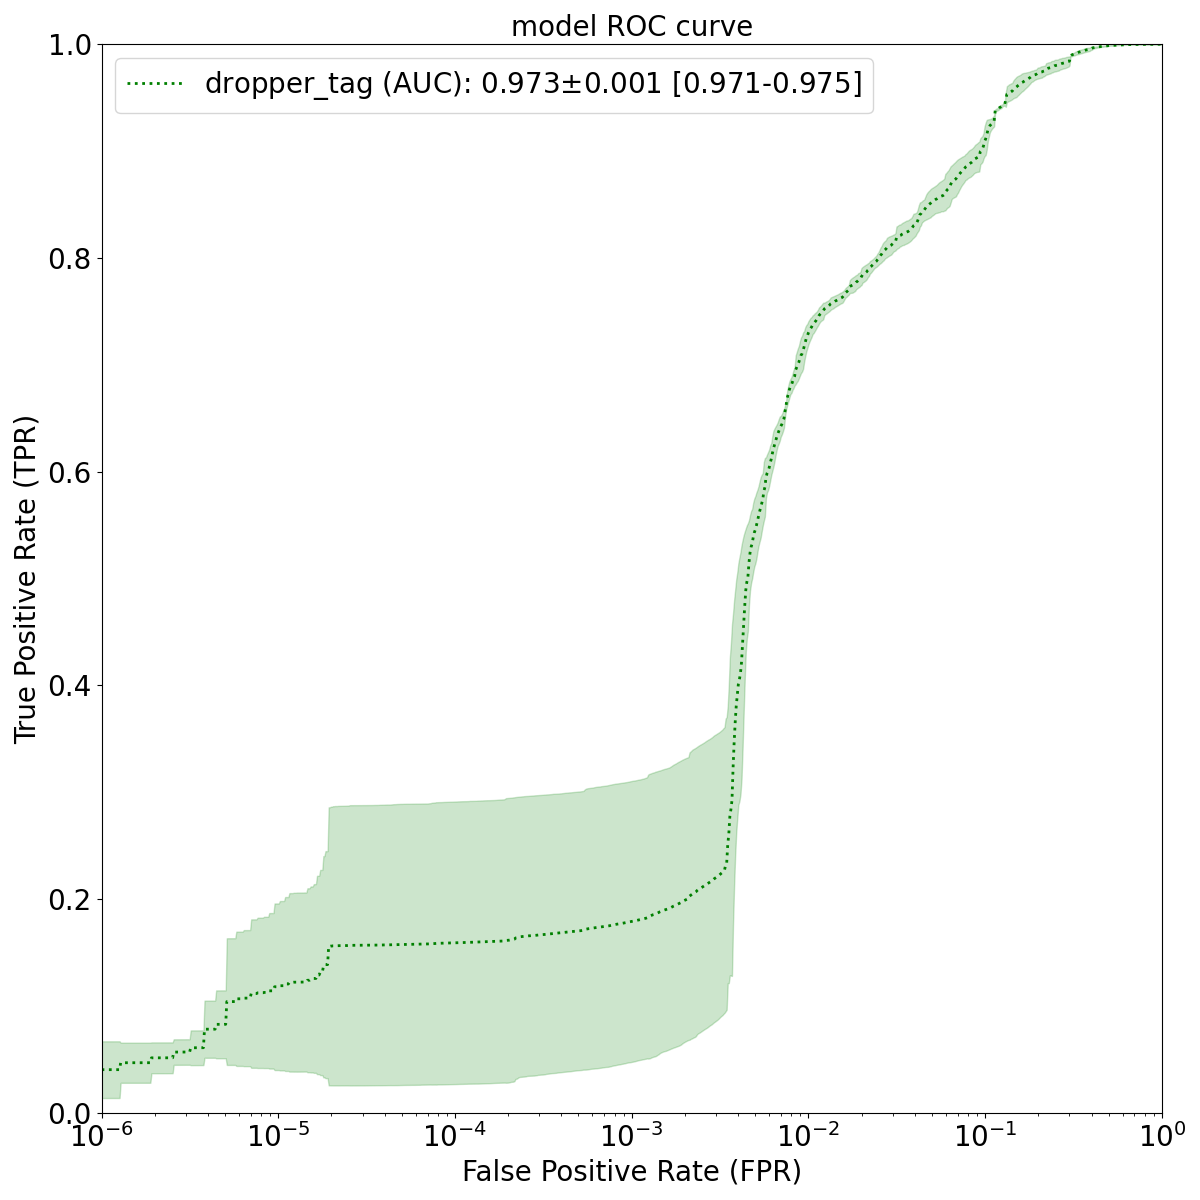
\includegraphics[width=0.6\textwidth]{./results/dropper_tag_roc_jointEmbedding.png}
        \vspace*{-0.2cm}
        \caption[Dropper Tag prediction task Joint Embedding ROC curve]{ROC curve and AUC statistics of \textBF{Joint Embedding} model for the \textbf{Dropper Tag}. The line represents the \textit{mean} TPR at a given FPR, while the shaded region represents the \textit{standard deviation}. Statistics were computed over \textBF{3} training runs, each with random parameter initialization.}
        \label{fig:dropperTagRocJointEmbedding}
    \end{figure}
}

\newcommand{\dropperTagRocProposedMethod}{
    \begin{figure}[h!]
        \vspace*{-0.5cm}
        \centering
        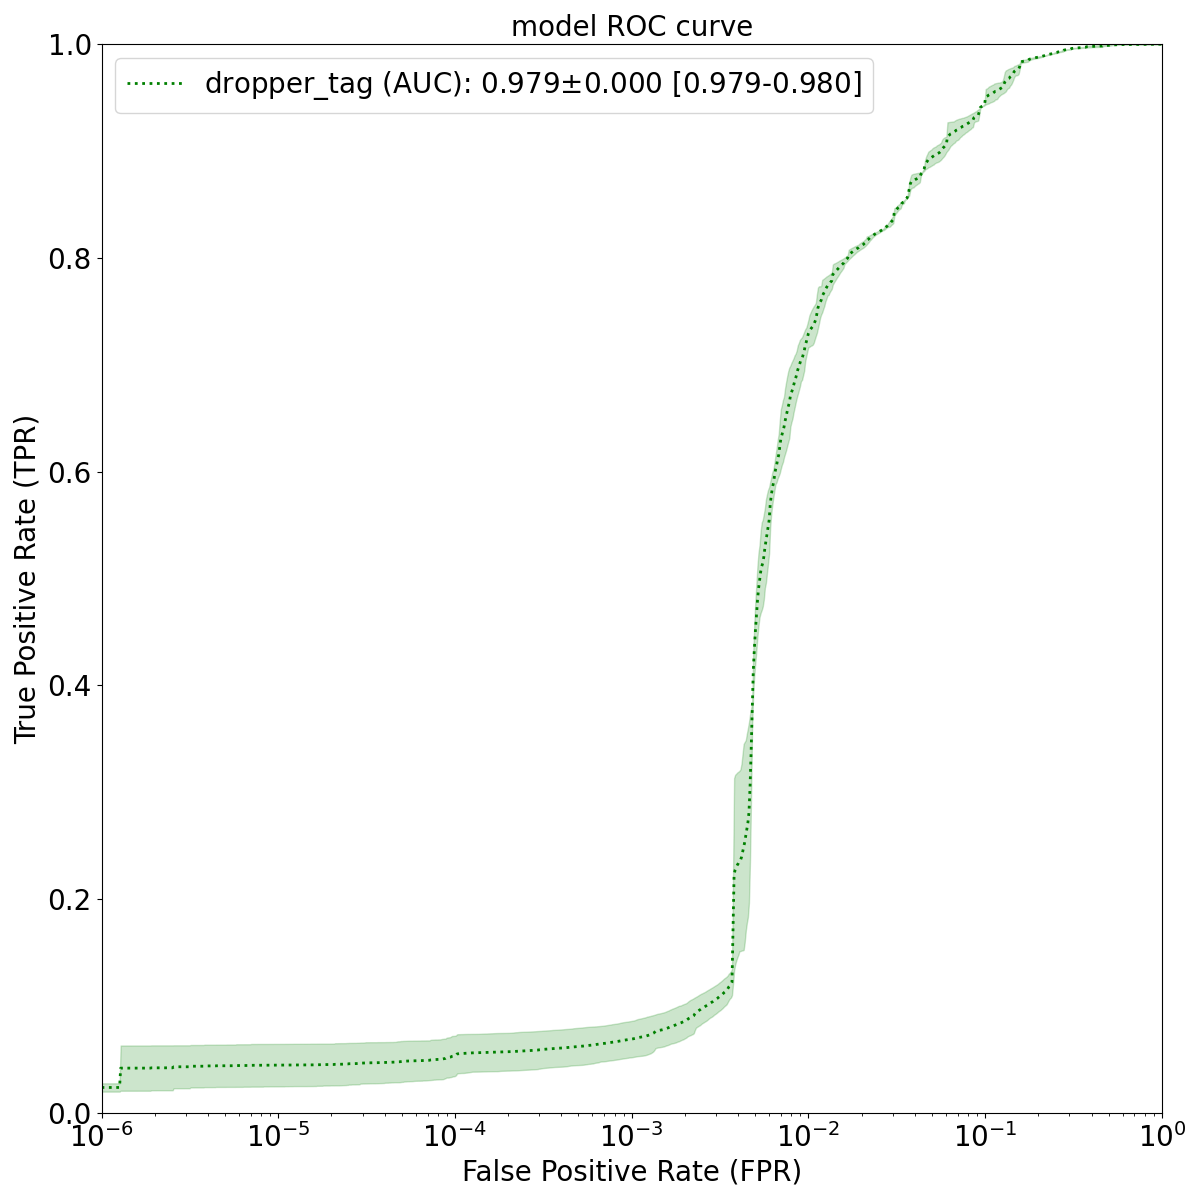
\includegraphics[width=0.6\textwidth]{./results/dropper_tag_roc_proposedModel.png}
        \vspace*{-0.2cm}
        \caption[Dropper Tag prediction task Proposed Model ROC curve]{ROC curve and AUC statistics of \textBF{Proposed Model} for the \textbf{Dropper Tag}. The line represents the \textit{mean} TPR at a given FPR, while the shaded region represents the \textit{standard deviation}. Statistics were computed over \textBF{3} training runs, each with random parameter initialization.}
        \label{fig:dropperTagRocProposedModel}
    \end{figure}
}
